\setcounter{chaptercntr}{6}

\sectionbreak \section*{
	\gostTitleFont
	\redline
	\thechaptercntr .
	АНАЛИЗ ПРЕДМЕТНОЙ ОБЛАСТИ И ПОСТАНОВКА ЗАДАЧИ
}

\titlespace

\subsection*{ 
	\gostTitleFont
	\redline
	\thechaptercntr .\thesubchaptercntr \spc
	Исходные данные для расчета экономического эффекта
} \addtocounter{subchaptercntr}{1}

\subtitlespace

{\gostFont
	
	
	\par \redline Любая разработка программного обеспечения, приложения или их модулей требует финансовых и человеческих ресурсов.
	
	\par \redline Задачей данного дипломного проекта является разработка нейронной сети типа многослойный персептрон на языке программирования С++.
	
	\par \redline Разработка программного продукта предусматривает проведение всех стадий проектирования и относится к первой группе сложности. 
	
	\par \redline Последовательность расчетов:
	
	\par \redline •  Расчёт объёма функций программных модулей.
	
	\par \redline •  Расчёт полной себестоимости криптографической защиты.
	
	\par \redline •  Расчёт цены и прибыли по программному продукту.
	
}

\subtitlespace

\subsection*{ 
	\gostTitleFont
	\redline
	\thechaptercntr .\thesubchaptercntr \spc
	Расчет объёма функций программного обеспечения
} \addtocounter{subchaptercntr}{1}

\subtitlespace

{\gostFont
	
	\par \redline Общий объём ПО определяется по формуле (6.1), исходя из объёма функций, реализуемых программой. 
	
	\formulaspace
	\par \redline $ V_0=\sum_{i=0}^{n}V_i$ \hfill (\thechaptercntr .\theformulacntr) \redline
	\formulaspace \addtocounter{formulacntr}{1}

	\par \redline где $V_0$ {--} общий объём ПО;
	
	\par \redline \wherespace $V_i$ {--} объём функций ПО;
	
	\par \redline \wherespace n {--} общее число функций.
	
	\par \redline В том случае, когда на стадии технико-экономического обоснования проекта невозможно рассчитать точный объём функций, то данный объём может быть получен на основании прогнозируемой оценки имеющихся фактических данных по аналогичным проектам, выполненным ранее, или применением нормативов по каталогу функций.
	
	\par \redline По каталогу функций на основании функций разрабатываемых криптографических модулей определяется общий объём. Также на основе зависимостей от организационных и технологических условий, был скорректирован объём на основе экспертных оценок.
	
	\par \redline Уточнённый объём ПО определяется по формуле (6.2).
	
	\formulaspace
	\par \redline $V_y=\sum_{i=0}^{n}V_yi$ \hfill (\thechaptercntr .\theformulacntr) \redline
	\formulaspace \addtocounter{formulacntr}{1}
	
	\par \redline где \wherespace $V_y$ {--} уточнённый объём ПО;
	
	\par \redline \wherespace $V_{yi}$ {--} уточнённый объём отдельной функции в строках исходного кода.
	
	\par \redline Перечень и объём функций модулей криптографии приведён в таблице \thechaptercntr .\thetablecntr .

	\par \redline \par \redline

	\begin{flushleft}
		\par \centering Таблица \thechaptercntr .\thetablecntr \spc {--} Перечень и объем функций программного обеспечения
	\end{flushleft}

	\begin{figure}
		\centering
		\def\svgwidth{\textwidth}
		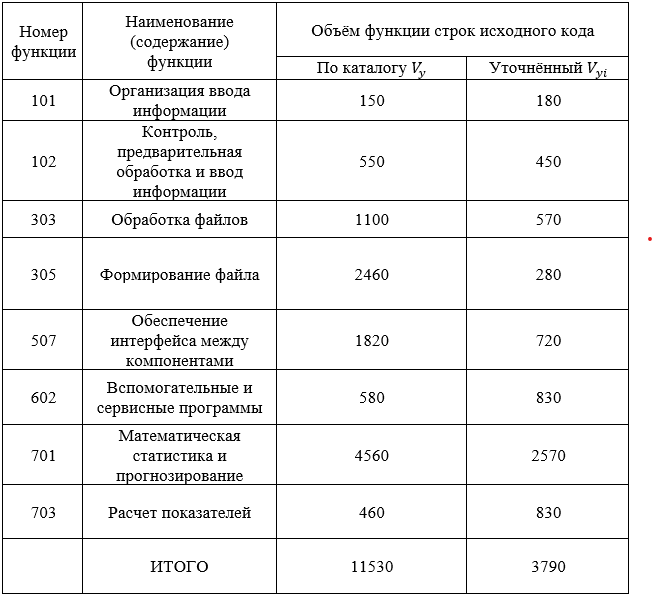
\includegraphics[scale=1.0]{images/elonomT1.png}
		\label{fig:ekonomT1}
	\end{figure}

	\par \redline Учитывая информацию, указанную в таблице \thechaptercntr .\thetablecntr \spc, о функциях разрабатываемого программного обеспечения, уточненный объем ПО ($V_{yi}$) составил 6430 строк исходного кода (LOC) вместо предполагаемого количества строк 11530. \addtocounter{tablecntr}{1}
	
	\par
}

\subtitlespace

\subsection*{ 
	\gostTitleFont
	\redline
	\thechaptercntr .\thesubchaptercntr \spc
	Расчет полной себестоимости программного продукта
} \addtocounter{subchaptercntr}{1}

\subtitlespace

{\gostFont
	
	\par \redline Стоимостная оценка программного средства у разработчика предполагает составление сметы затрат, которая включает следующие статьи расходов:
	
	\par \redline • заработную плату исполнителей (основную – ЗПо и дополнительную – ЗПд);
	\par \redline •	отчисления на социальные нужды (Рсоц);
	\par \redline •	материалы и комплектующие изделия (Рм);
	\par \redline •	спецоборудование (Рс);
	\par \redline •	машинное время (Рмв);
	\par \redline •	расходы на научные командировки (Рнк):
	\par \redline •	прочие прямые расходы (Рпр);
	\par \redline •	накладные расходы (Рнр);
	\par \redline •	затраты на освоение и сопровождение программного средства(Ро и Рсо).
	
	\par \redline Полная себестоимость (Сп) разработки программного продукта (ПП) рассчитывается как сумма расходов по всем статьям с учетом рыночной стоимости аналогичных продуктов.
	
	\par \redline Основной статьей расходов на создание ПП является заработная плата разработчиков (исполнителей) , в число которых принято включать инженеров-программистов, руководителей проекта, системных архитекторов, дизайнеров, разработчиков баз данных, Web-мастеров и других специалистов, необходимых для решения специальных задач в команде.
	 
	\par \redline Расчёт заработной платы разработчиков ПП начинается с определения:
	\par \redline •	Продолжительности времени разработки Фрв, которое устанавливается экспертным путем с учётом сложности, новизны ПП и фактически затраченного времени. В данном дипломном проекте Фрв = 31 дней.
	\par \redline •	Количества разработчиков ПП. В данном дипломном проекте один разработчик (инженер-программист 10 разряда).
	Заработная плата работника будет включать:
	\par \redline 1. оклад;
	\par \redline 2. стимулирующие и компенсирующие надбавки и премию, а именно:
	\par \redline \hspace{15mm} •	надбавка за работу по контракту;
	\par \redline \hspace{15mm} •	надбавка за характер труда;
	\par \redline \hspace{15mm} •	премия в размере 5 \% от суммы оклада работника;
	\par \redline \hspace{15mm} •	надбавка за стаж работы (в \% от базовой ставки);
	\par \redline \hspace{15mm} •	надбавка за высокие достижения в труде.
	\par \redline Для расчета месячной заработной платы используем формулу (6.3):

	\begin{equation}
		\textrm{ЗПмес = Оклад + стимулирующие выплаты + компенсирующие выплаты} 
	\end{equation}
	
	\par \redline Тарифный оклад рассчитывается по формуле (6.4):
	
	\begin{equation}
		\textrm{Тариф. Оклад = Базовая ставка * тарифный коэффициент,}
	\end{equation}
	
	\par \redline После того, как мы определим месячную заработную плату специалиста, необходимо пересчитать её на фактическое число дней работы конкретного специалиста над проектом (ПП). В нашем случае фактическое количество дней – 31.
	\par \redline Поэтому заработную плату каждого исполнителя определяем по формуле (6.5):
	
	\begin{equation}
		\textrm{ЗПспец = Зарплата месячная / 21 * Фрв,}
	\end{equation}
	
	\par \redline где 21 – среднее количество рабочих дней в месяце; 
    \par \redline \hspace{7mm}Фрв – фонд рабочего времени исполнителя (дни).
	\par \redline Рассчитаем заработную плату исполнителей проекта и результаты занесем в таблицу 4.2.
	
	\begin{table}[]
		\centering
		\begin{tabular}{|c|c|c|c|c|ccc|}
		\hline
		\multirow{2}{*}{Категория работников} &
		  \begin{sideways} \multirow{2}{*}{Разряд} \end{sideways} &
		  \multirow{2}{*}{Тарифный коэффициент (Тк)} &
		  \multirow{2}{*}{Фэфф.р.в.,(дн.)} &
		  \multirow{2}{*}{Коэффициент премии (Кпр)} &
		  \multicolumn{3}{c|}{Заработная плата, бел. руб} \\ \cline{6-8} 
							&   &      &    &     & \multicolumn{1}{c|}{Основная} & \multicolumn{1}{c|}{Дополнительная} & Всего   \\ \hline
		Инженер-программист & 8 & 1,57 & 70 & 1,4 & \multicolumn{1}{c|}{1748,41}  & \multicolumn{1}{c|}{262,26}         & 2010,70 \\ \hline
		Итого               & - & -    & -  & -   & \multicolumn{1}{c|}{1748,41}  & \multicolumn{1}{c|}{262,26}         & 2010,70 \\ \hline
		\end{tabular}
		\end{table}

	\par 
}
